%! Author = alanmiranda
%! Date = 14/11/2022

\subsection{Materiais}\label{subsec:mat_materiais}
    \indent Os materiais utilizados para a realização desta prática foram:
        \begin{table}[h]
        \label{tab:materiais}
        \centering
        \begin{tabular}{|c|c|}
            \hline
            \textbf{Material} & \textbf{Quantidade} \\
            \hline
            Solução de NaOH 0,1 mol/L & 10 mL \\
            \hline
            Solução de HCl 0,1 mol/L & 10 mL \\
            \hline
            Solução de CH$_3$COOH 0,1 mol/L & 10 mL \\
            \hline
            Solução de NH$_4$OH 0,1 mol/L & 10 mL \\
            \hline
            Indicador ácido: Fenolftaleína & 0,15 mL \\
            \hline
            Indicador universal: Azul de bromotimol & 0,15 mL \\
            \hline
            Indicador universal: Alaranjado de metila & 0,15 mL \\
            \hline
            Indicador universal: Papeis de tornassol azul e vermelho & 3 pedaços/amostra \\
            \hline
            Água Sanitária & 10 mL \\
            \hline
            Detergente & 10 mL \\
            \hline
            Suco de limão & 10 mL \\
            \hline
            Suco de Uva & 10 mL \\
            \hline
        \end{tabular}
            \caption{Materiais utilizados neste relatório}
    \end{table}\\
    \newpage
    \indent E a seguinte bancada de trabalho:\\
    \begin{figure}[h]
        \centering
        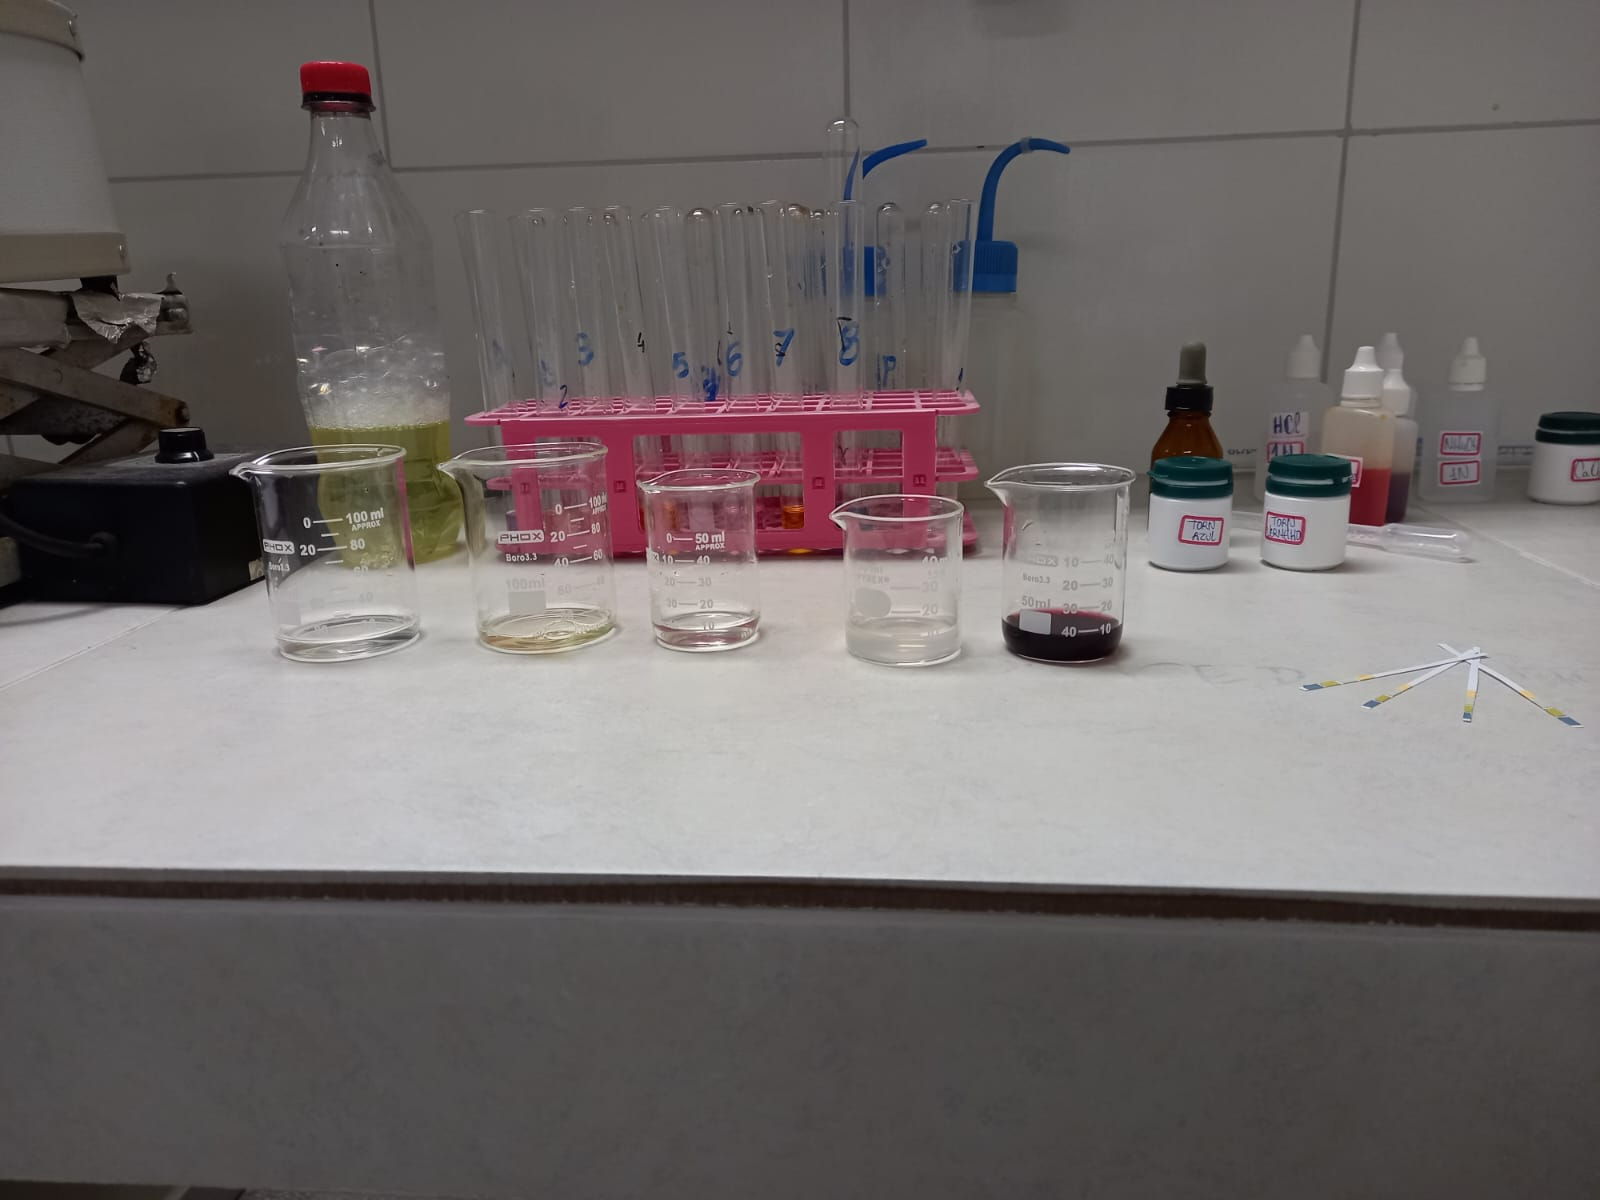
\includegraphics[scale=0.25]{pictures/bancada.jpeg}
        \caption{Bancada de trabalho utilizada para a realização desta prática}\label{fig:figure1}
    \end{figure}\\

    \indent E os materiais de bancada de trabalho utilizadps para a realização desta prática foi composta por:
    \begin{enumerate}
        \item \textbf{10 Tubos de Ensaio} - Utilizados para o preparo das soluções e testes dos indicadores.
        \item \textbf{1 Espátula} - Utilizada para a retirada de amostras das soluções.
        \item \textbf{1 pipeta de 25 mL} - Utilizada para a retirada de amostras das soluções.
        \item \textbf{2 Beckers de 100 mL} - Utilizados para o preparo das soluções.
        \item \textbf{2 Becker de 50 mL} - Utilizado para o preparo das soluções.
        \item \textbf{Estante para tubos de ensaio} - Utilizada para a organização dos tubos de ensaio.
        \item \textbf{Funil de vidro} - Utilizado para o preparo das soluções.
        \item \textbf{Bureta de vidro} - Utilizada para o preparo das soluções.
    \end{enumerate}

    \subsubsection{Indicadores}\label{subsubsec:mat_materiais_indicadores}
    \indent Muitas substâncias apresentam cores características em determinadas condições, e este é o caso dos indicadores de pH. A exemplo dos indicadores ácidos, estes liberam íons hidroxila (OH$^-$) em solução aquosa, e, portanto, apresentam cores características em soluções ácidas.
    Os indicadores ácidos mais comuns são a fenolftaleína e o bromotimol.
    A fenolftaleína apresenta uma coloração rosa em soluções ácidas e uma coloração incolor em soluções básicas.
    O bromotimol apresenta uma coloração amarela em soluções ácidas e uma coloração azul em soluções básicas.
    Os indicadores ácidos são muito utilizados em laboratórios de química, pois são baratos e fáceis de se obter.
    Além disso, são muito estáveis e apresentam uma boa faixa de pH de coloração.\\
    Portanto, os indicadores ácidos apresentam cores características em soluções ácidas.
    O mesmo ocorre com indicadores básicos e indicadores universais, pois tais compostos irão apresentar cores diferentes em soluções ácidas e básicas.
    Com tudo a depender das concentrações dos íons de (H$^+$) e de (OH$^-$) na solução.

    \subsection{Métodos}\label{subsec:mat_metodos}
        \indent A experimentação foi realizada seguindo conforme o especificado a seguir:

    \subsubsection{Experimento 1}\label{subsubsec:mat_metodos_exp1}
        \indent Para a realização do experimento 1, foram preparados os tubos de ensaio, cada tubo foi identificado seguindo a numeração de 1 a 8, preparado com suas respectivas soluções para a realização dos testes.\\

        \begin{figure}[h]
            \centering
            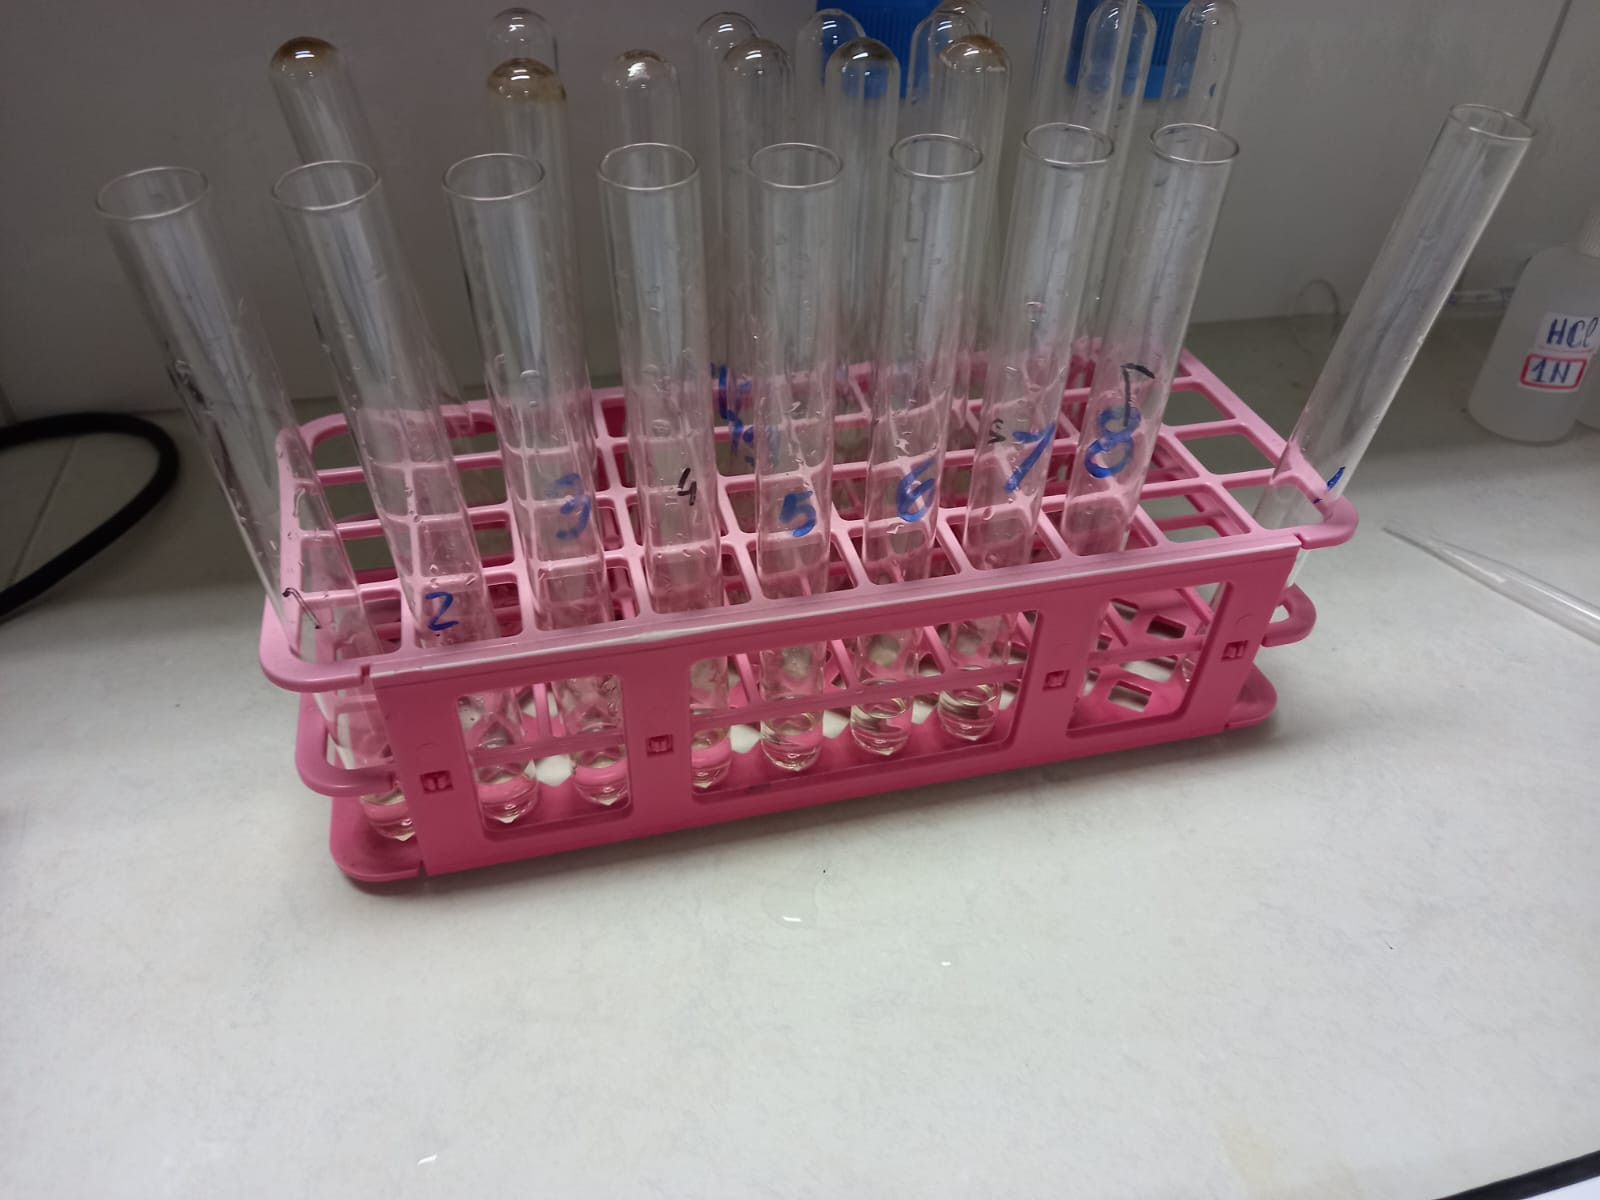
\includegraphics[scale=0.25]{pictures/tubos.jpeg}
            \caption{Tubos de ensaio utilizados para a realização do experimento 1}\label{fig:figure2}
        \end{figure}

        \indent Em suma, os tubos de ensaio foram preparados e testados com os indicadores, seguindo a tabela a seguir, cada experimentação será descrita detalhadamente posteriormente.\\

        \newpage

        \begin{table}[h]\label{tab:tubos}
            \label{tab:experimento1}
            \centering
            \begin{tabular}{|c|c|c|c|c|c|c|c|}
                \hline
                \textbf{Tubo} & \textbf{Solução} & \textbf{Indicador} & \textbf{Cor Apresentada}\\
                \hline
                1 & Solução de NaOH 0,1 mol/L & Papel Tornassol - Azul & Cristalino azulado \\
                \hline
                2 & Solução de HCl 0,1 mol/L & Papel Tornassol - Azul & Cristalino azulado \\
                \hline
                3 & Solução de CH$_3$COOH 0,1 mol/L & Alaranjado de Metila & cor\\
                \hline
                4 & Solução de NH$_4$OH 0,1 mol/L & Alaranjado de Metila & Branco \\
                \hline
                5 & Solução de HCl 0,1 mol/L & Fenolftaleína & Rosa \\
                \hline
                6 & Solução de NaOH 0,1 mol/L & Fenolftaleína & Incolor \\
                \hline
                7 & Solução de CH$_4$COOH 0,1 mol/L & Azul de Bromotimol & Azul \\
                \hline
                8 & Solução de NH$_4$OH 0,1 mol/L & Azul de Bromotimol & Branco \\
                \hline
            \end{tabular}
            \caption{Tabela de experimento 1}
        \end{table}

        \indent O primeiro tubo foi preparado com a solução de NaOH 0,1 mol/L, e foi testado com o indicador de pH, o papel de tornassol azul, o qual apresentou uma cor cristalina azulada.\\

        \indent O segundo tubo foi preparado com a solução de HCl 0,1 mol/L, e foi testado com o indicador de pH, o papel de tornassol vermelho, o qual apresentou uma cor cristalina azulada, os comportamentos dos tubos 1 e 2 podem ser visualizados conforme a figura a seguir:\\

        \begin{figure}[h]
            \centering
            \subfloat[\centering Teste do indicador de pH com as soluções de NaOH e HCl de 0,1 mol/L\label{fig:figure3}]{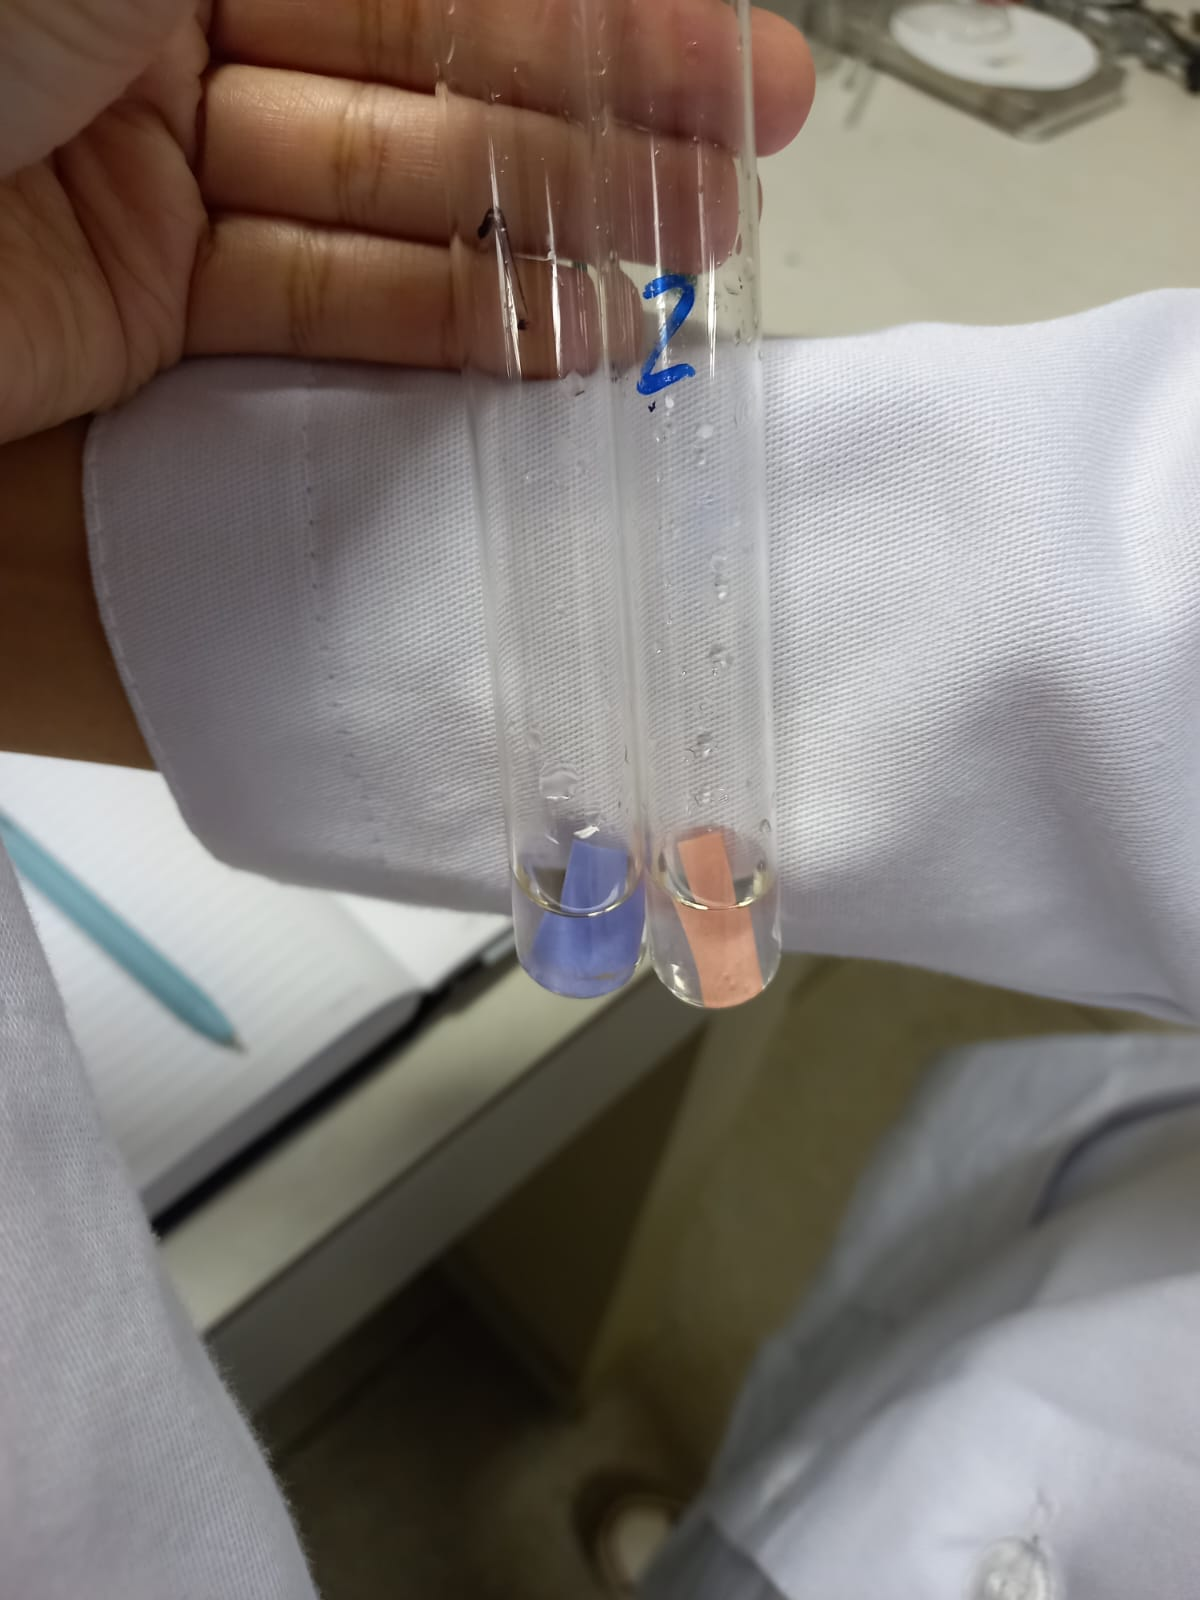
\includegraphics[scale=0.16]{pictures/tubo1e2pre.jpeg}}
            \qquad
            \subfloat[\centering Teste com as soluções com a adição dos papéis azul e vermelho em ambos os tubos. \label{fig:figure4}]{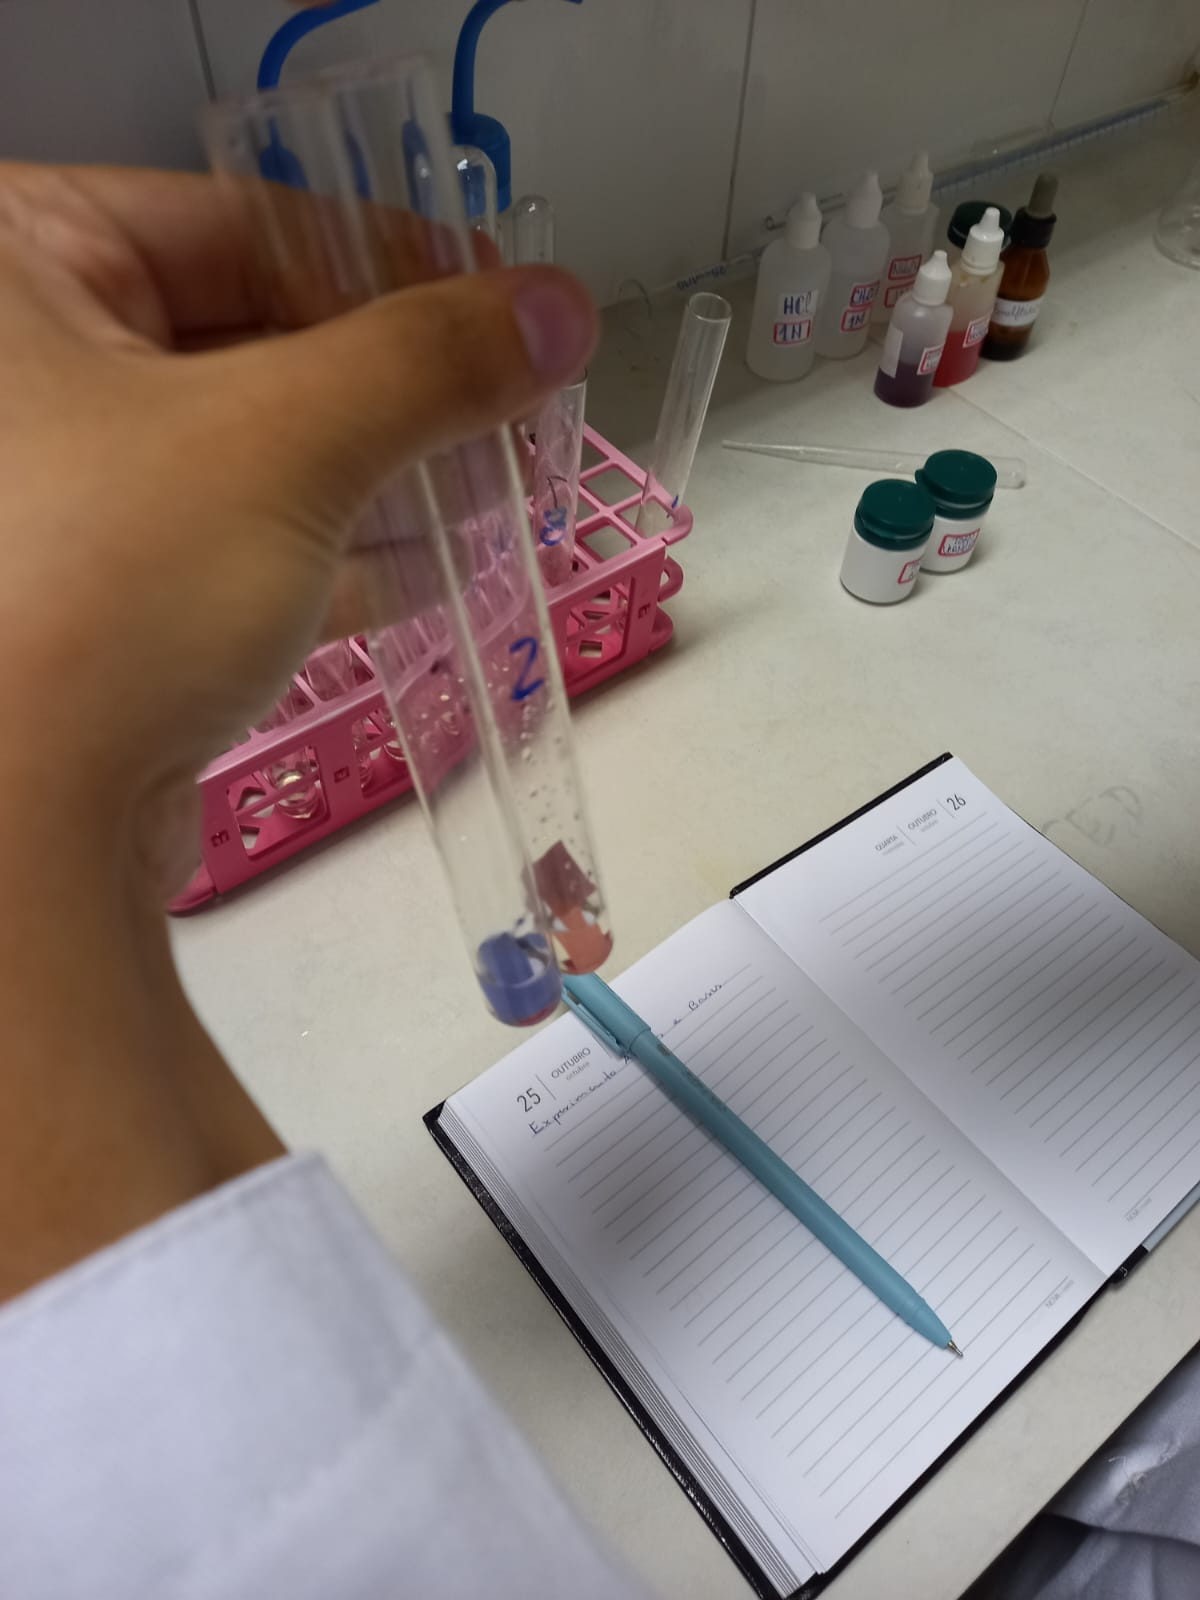
\includegraphics[scale=0.16]{pictures/tubo1e2pos.jpeg}}
            \caption{Teste do indicador de pH, o papel de tornassol azul e vermelho, nos tubos 1 e 2}\label{fig:experimento11}
        \end{figure}

        \indent O papel tornassol é muito utilizado em avaliações qualitativas de pH, é conhecido que seu comportamento é de tornar-se vermelho em soluções com pH abaixo de 4,7 e azul em soluções com pH acima de 8,3. Foi observado que, quando um papel azul é exposto à uma solução ácida, este se torna vermelho, e quando exposto à uma solução básica, nada acontece, e quando um papel vermelho é exposto em uma solução básica, este torna-se azul, mas quando exposto à solução ácida, nada acontece.
        \newpage

        \indent O terceiro tubo foi preparado com a solução de CH$_3$COOH 0,1 mol/L, e foi testado com o indicador de pH, o alaranjado de metila, o qual apresentou uma cor alaranjada.

        \begin{figure}[h]
            \centering
            \subfloat[\centering Teste do indicador de pH com a solução de CH$_3$COOH de 0,1 mol/L\label{fig:figure5}]{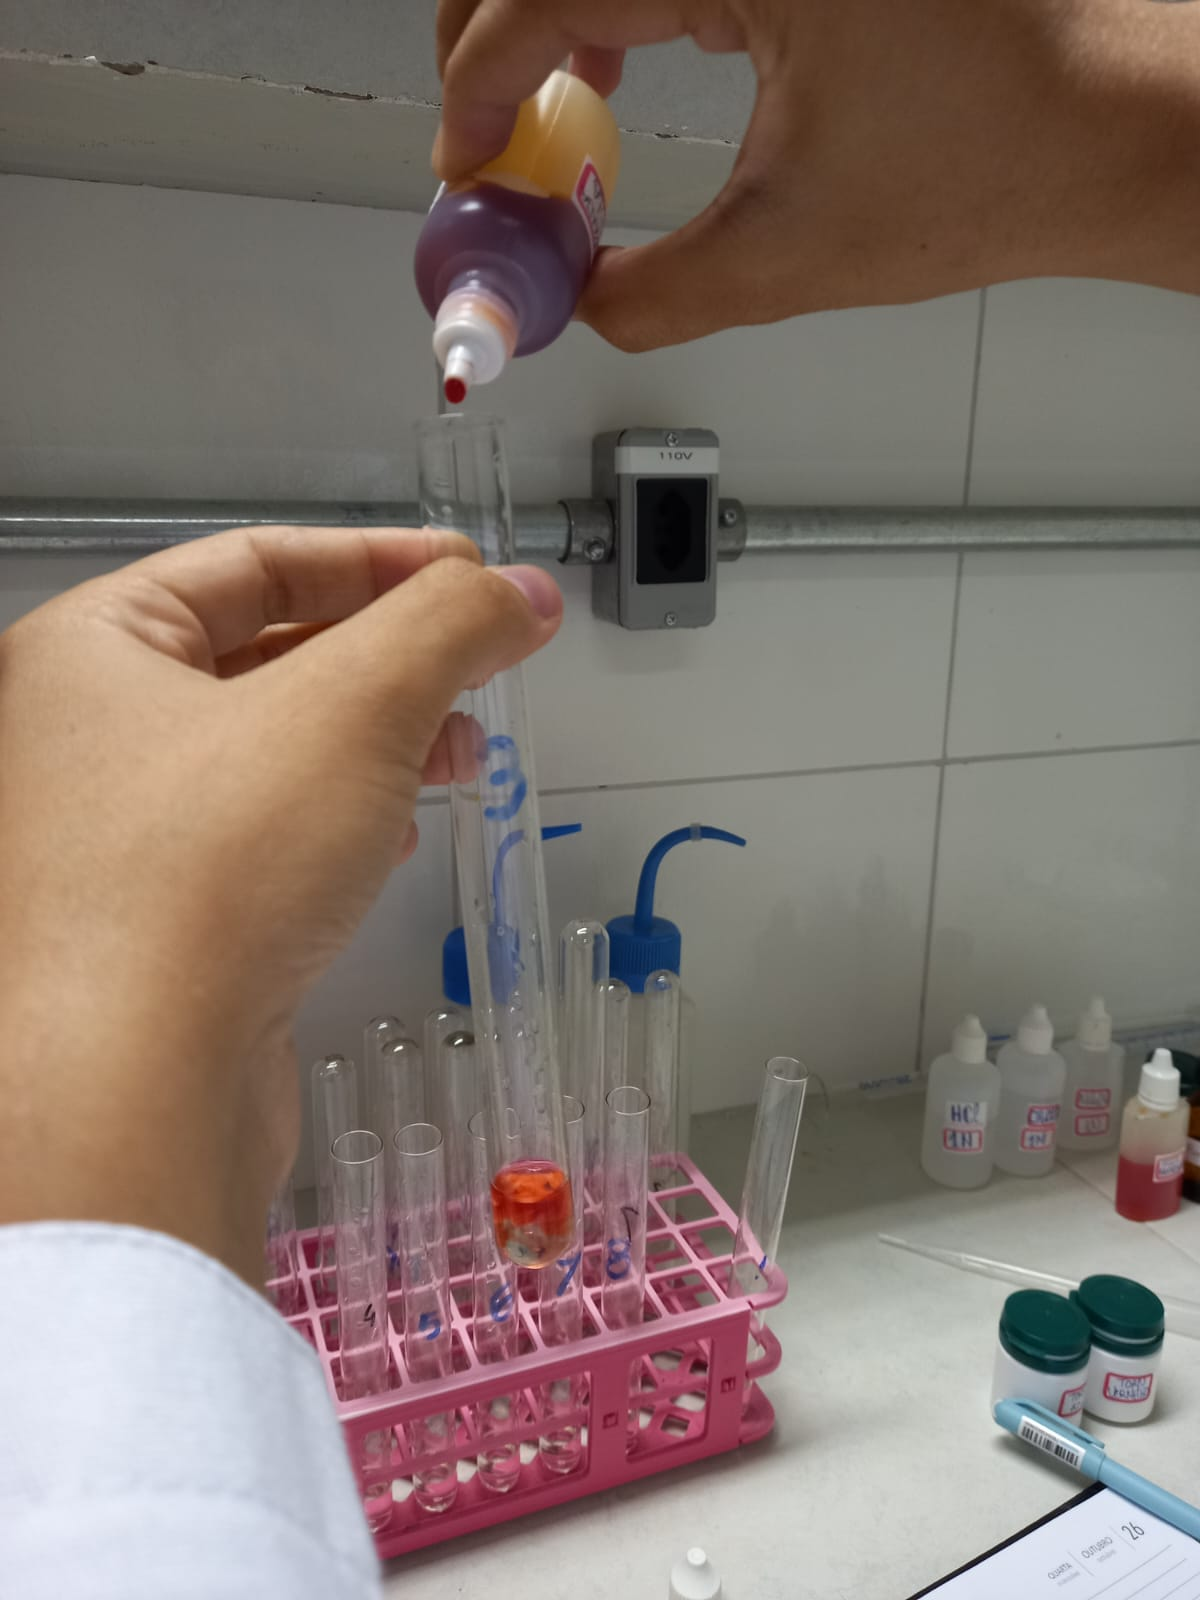
\includegraphics[scale=0.16]{pictures/tubo3pre.jpeg}}
            \qquad
            \subfloat[\centering A coloração apresentadapelo indicador foi alaranjada.\label{fig:figure6}]{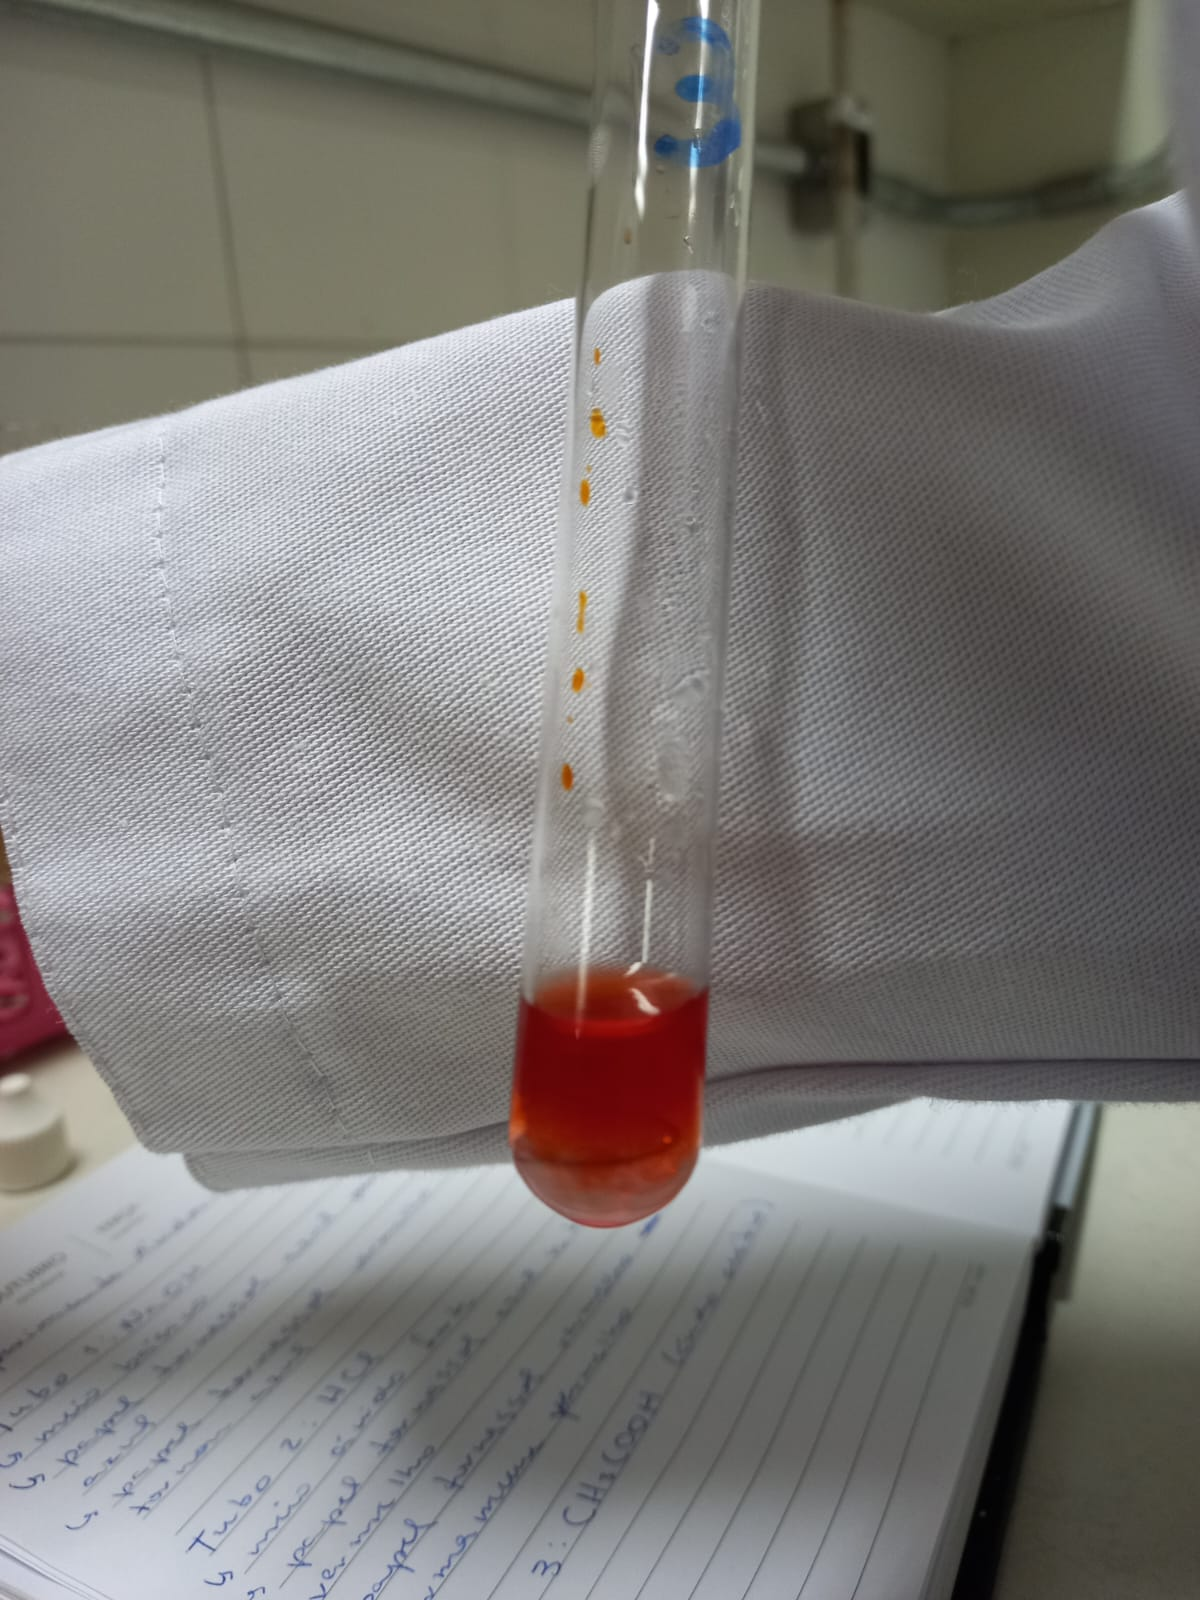
\includegraphics[scale=0.16]{pictures/tubo3pos.jpeg}}\label{fig:experimento12}
        \end{figure}

        \newpage

        \indent O quarto tubo foi preparado com a solução de NH$_4$OH 0,1 mol/L, e foi testado com o indicador de pH, o alaranjado de metila, o qual apresentou uma cor branca.

        \begin{figure}[h]
            \centering
            \subfloat[\centering Teste do indicador de pH com a solução de NH$_4$OH de 0,1 mol/L\label{fig:figure7}]{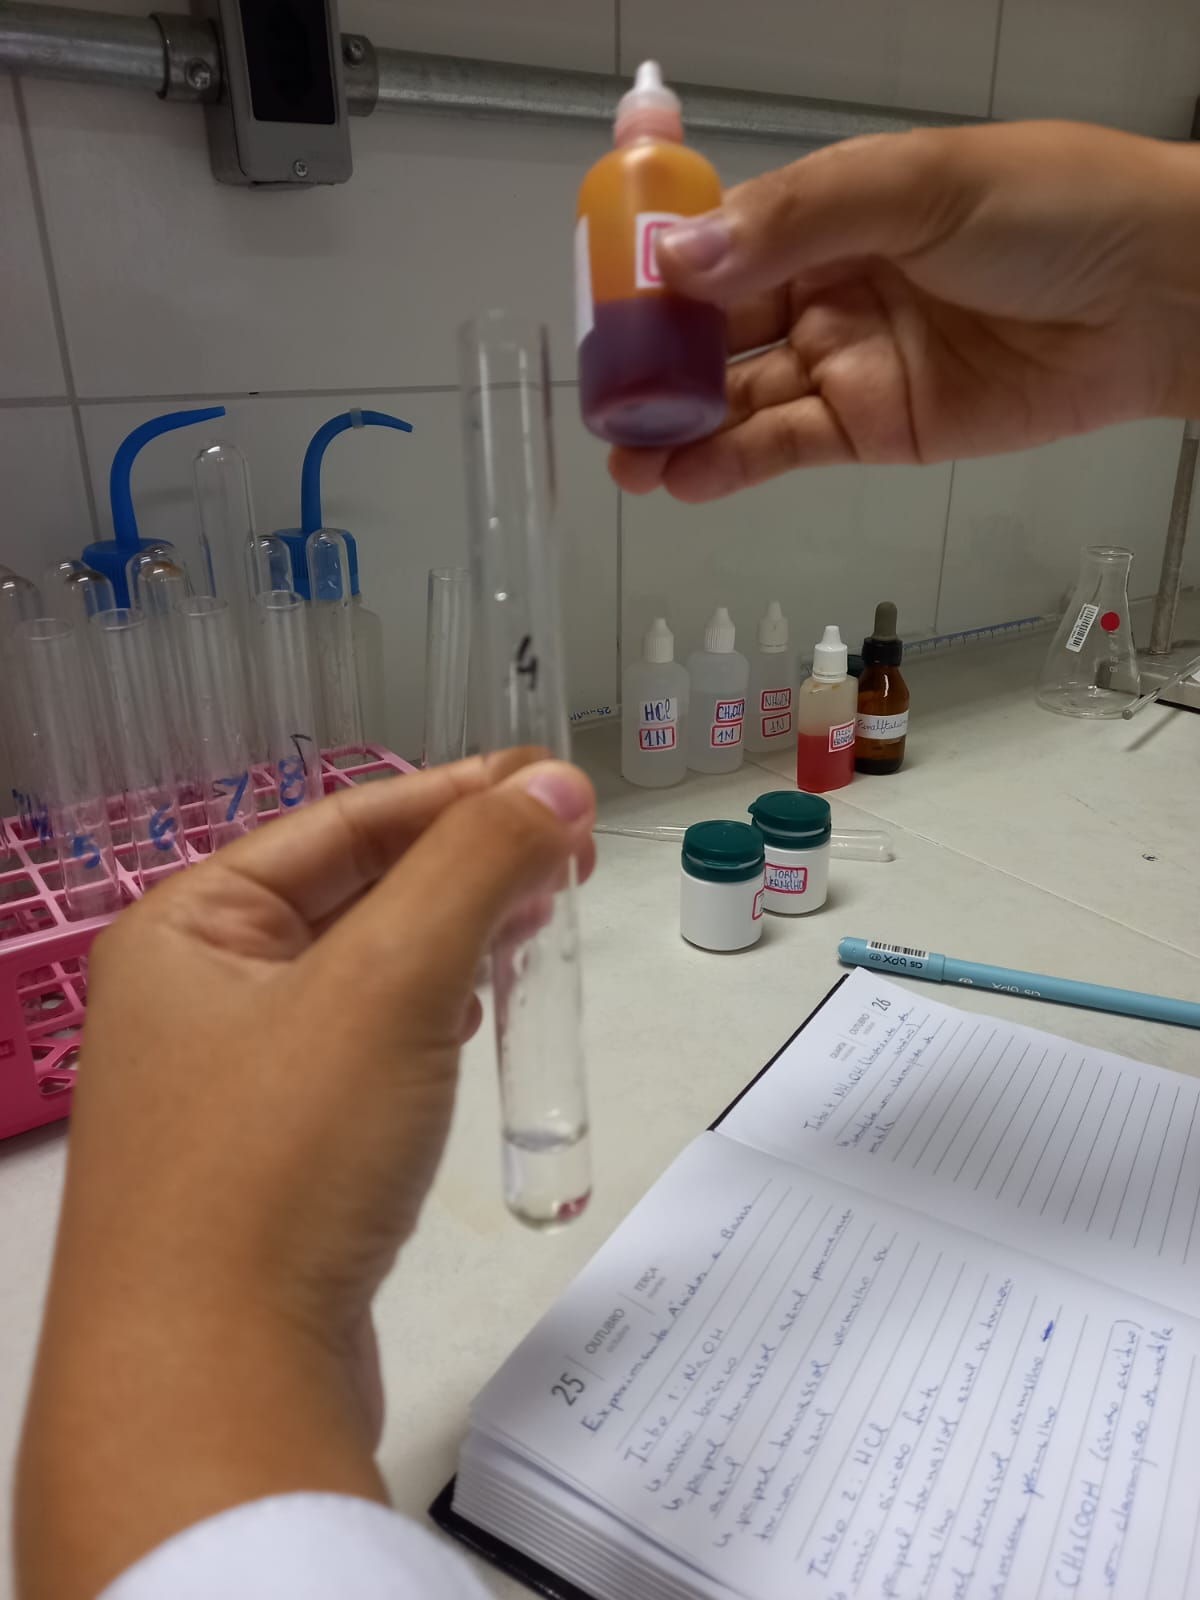
\includegraphics[scale=0.16]{pictures/tubo4pre.jpeg}}
            \qquad
            \subfloat[\centering A coloração apresentada pelo indicador foi branca. \label{fig:figure8}]{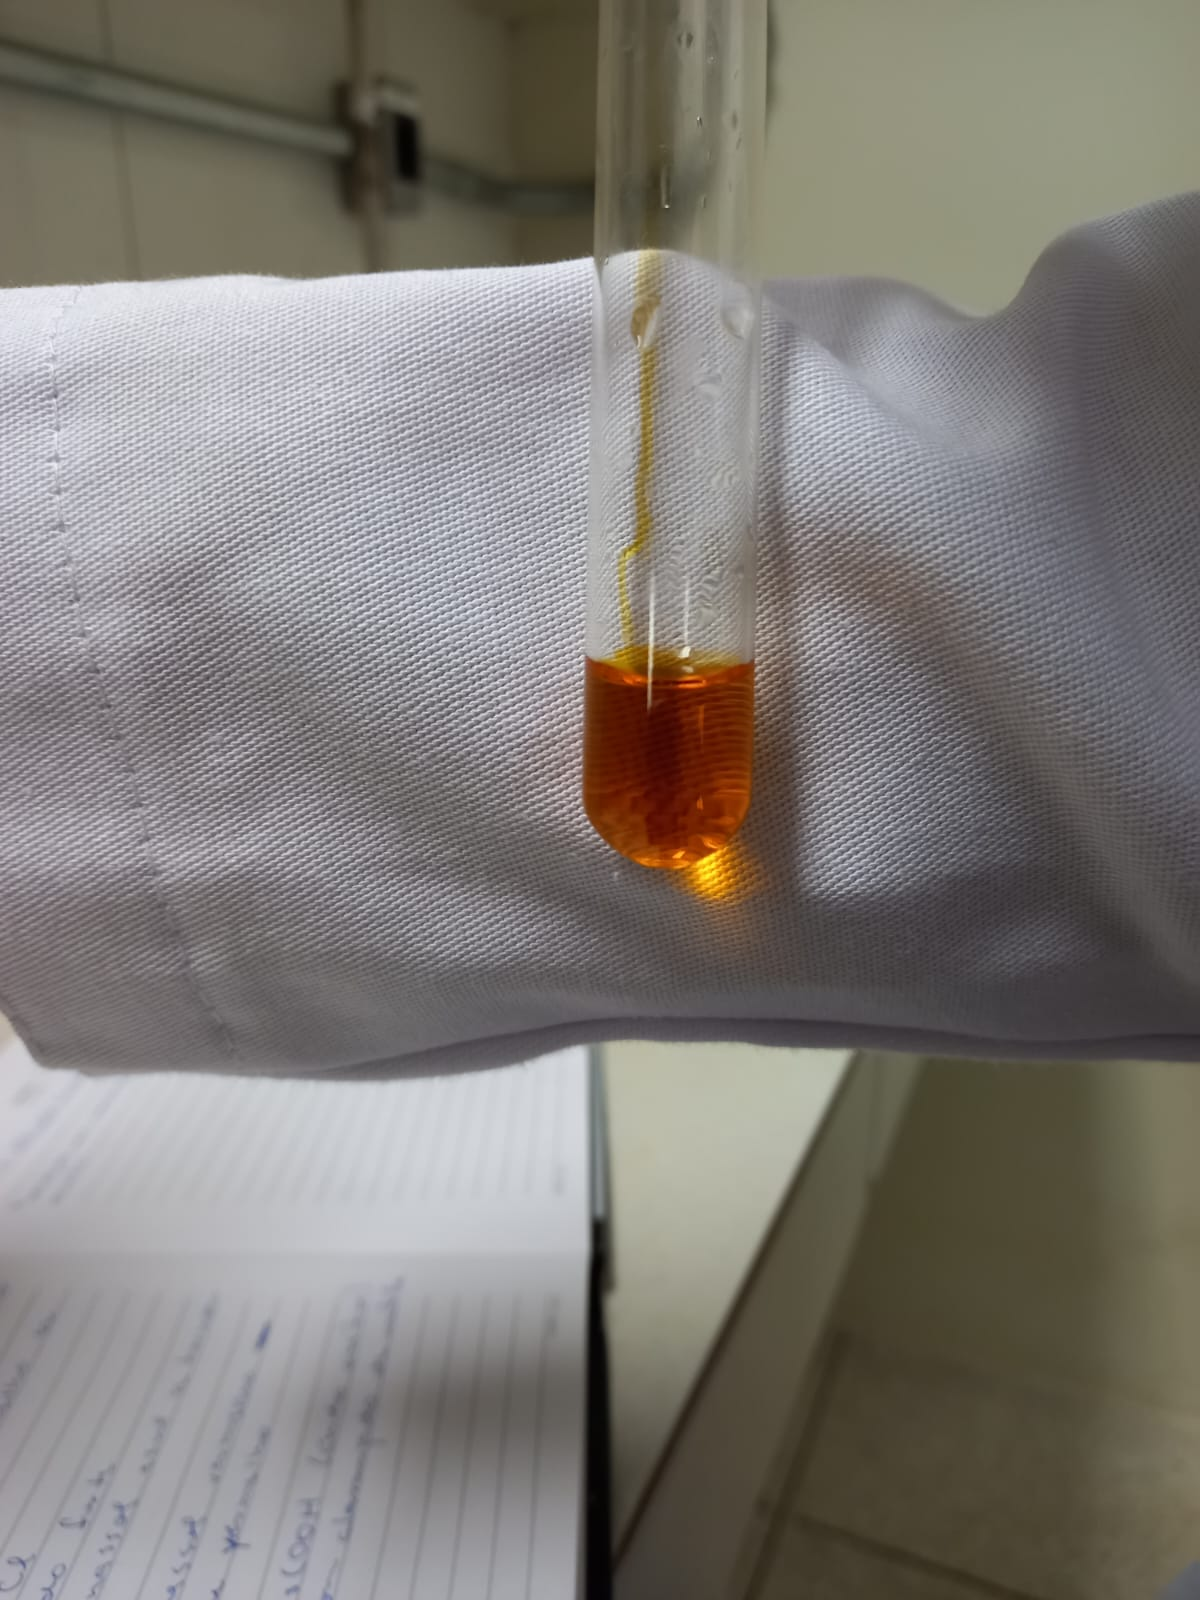
\includegraphics[scale=0.16]{pictures/tubo4pos.jpeg}}\label{fig:experimento13}
        \end{figure}

        \newpage

        \indent O quinto tubo foi preparado com a solução de HCl 0,1 mol/L, e foi testado com o indicador de pH, a fenolftaleína, o qual apresentou uma cor rosa.

        \begin{figure}[h]
            \centering
                \subfloat[\centering Teste do indicador de pH com a solução de HCl de 0,1 mol/L\label{fig:figure9}]{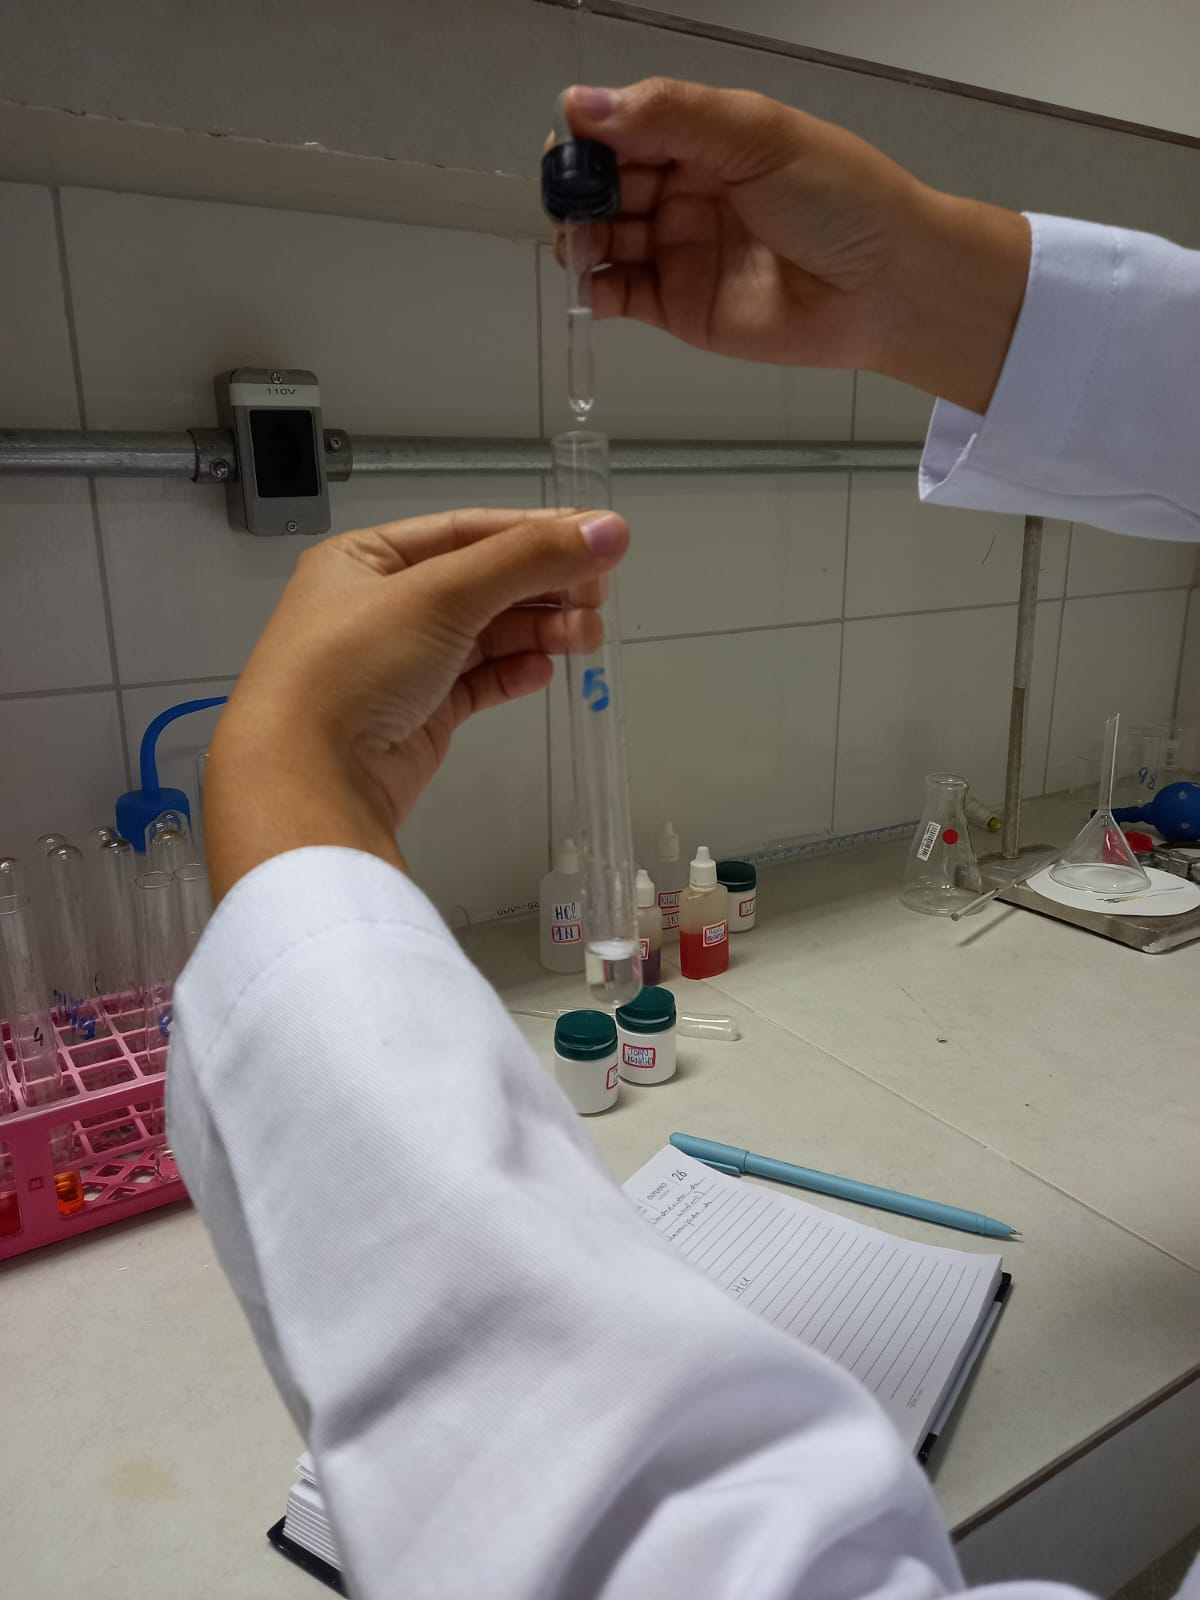
\includegraphics[scale=0.14]{pictures/tubo5pre.jpeg}}
                \qquad
                \subfloat[\centering A coloração apresentada pelo indicador foi rosa.\label{fig:figure10}]{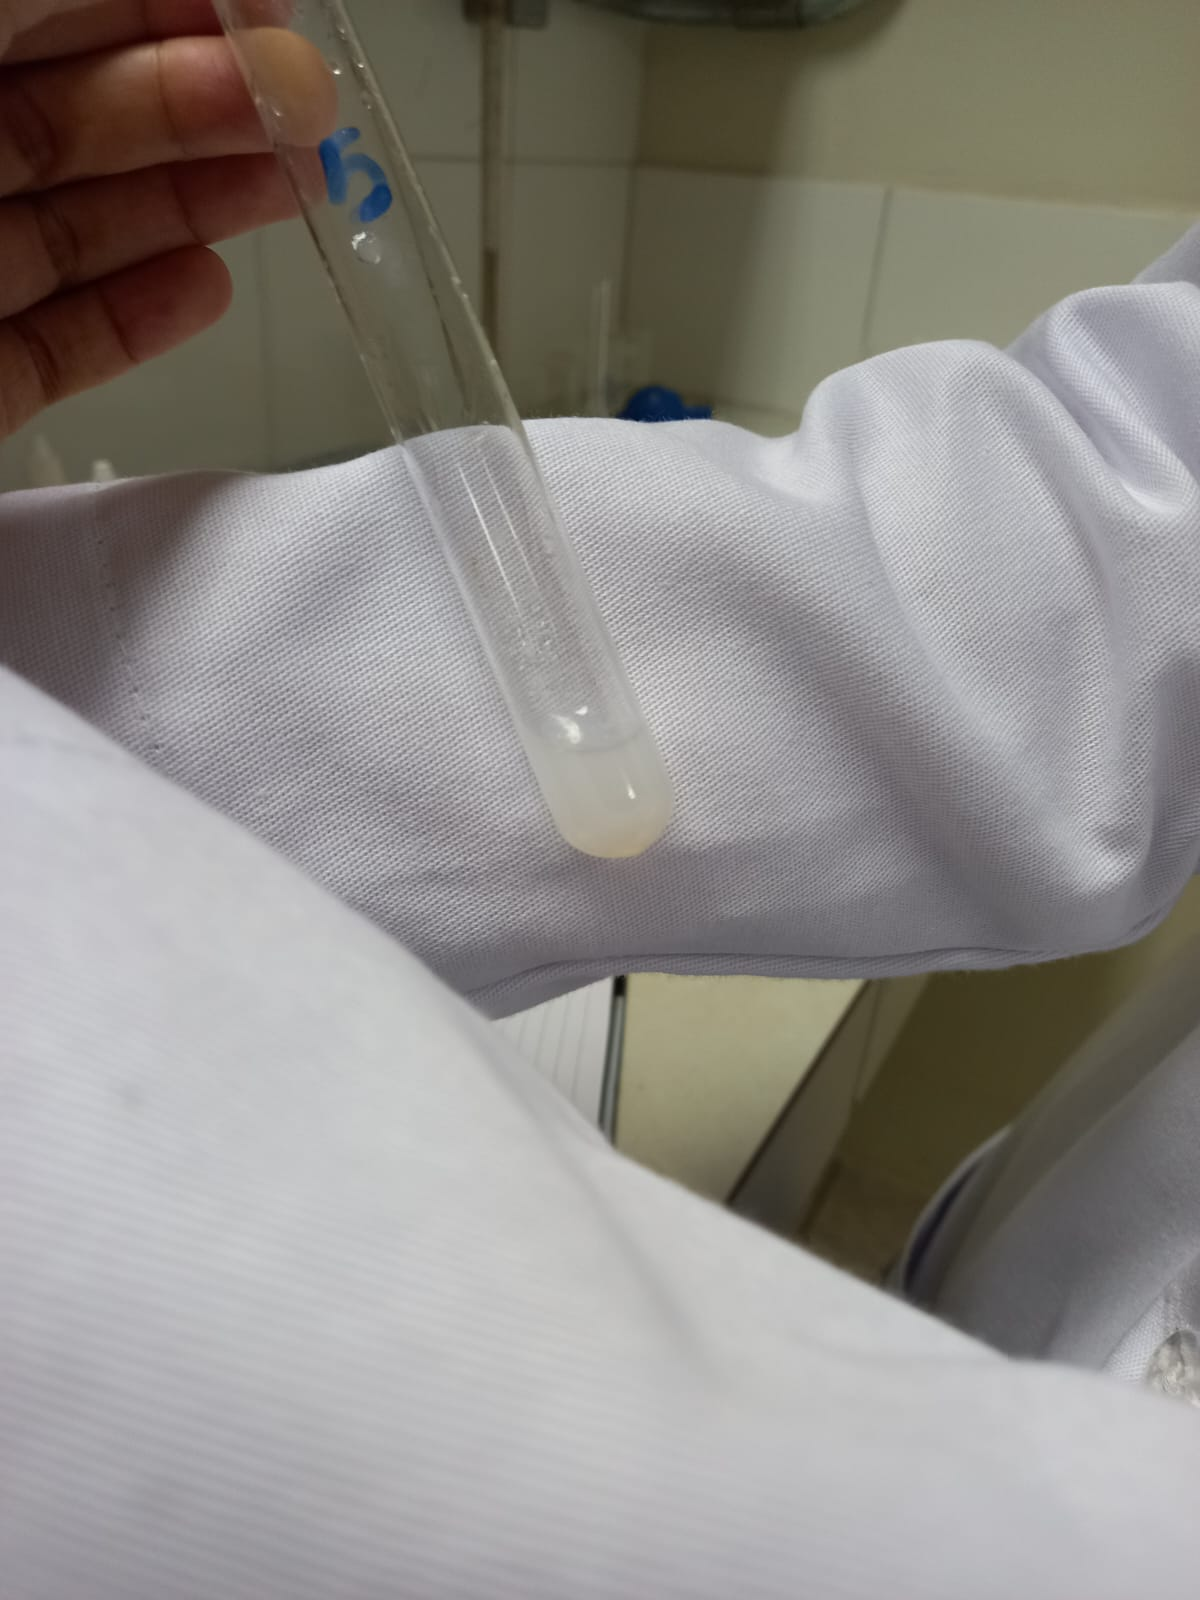
\includegraphics[scale=0.14]{pictures/tubo5pos.jpeg}}\label{fig:experimento14}
        \end{figure}

        \newpage

        \indent O sexto tubo foi preparado com a solução de NaOH 0,1 mol/L, e foi testado com o indicador de pH, a fenolftaleína, o qual apresentou uma solução incolor.
        \begin{figure}[h]
            \centering
            \subfloat[\centering Teste do indicador de pH com a solução de NaOH de 0,1 mol/L\label{fig:figure11}]{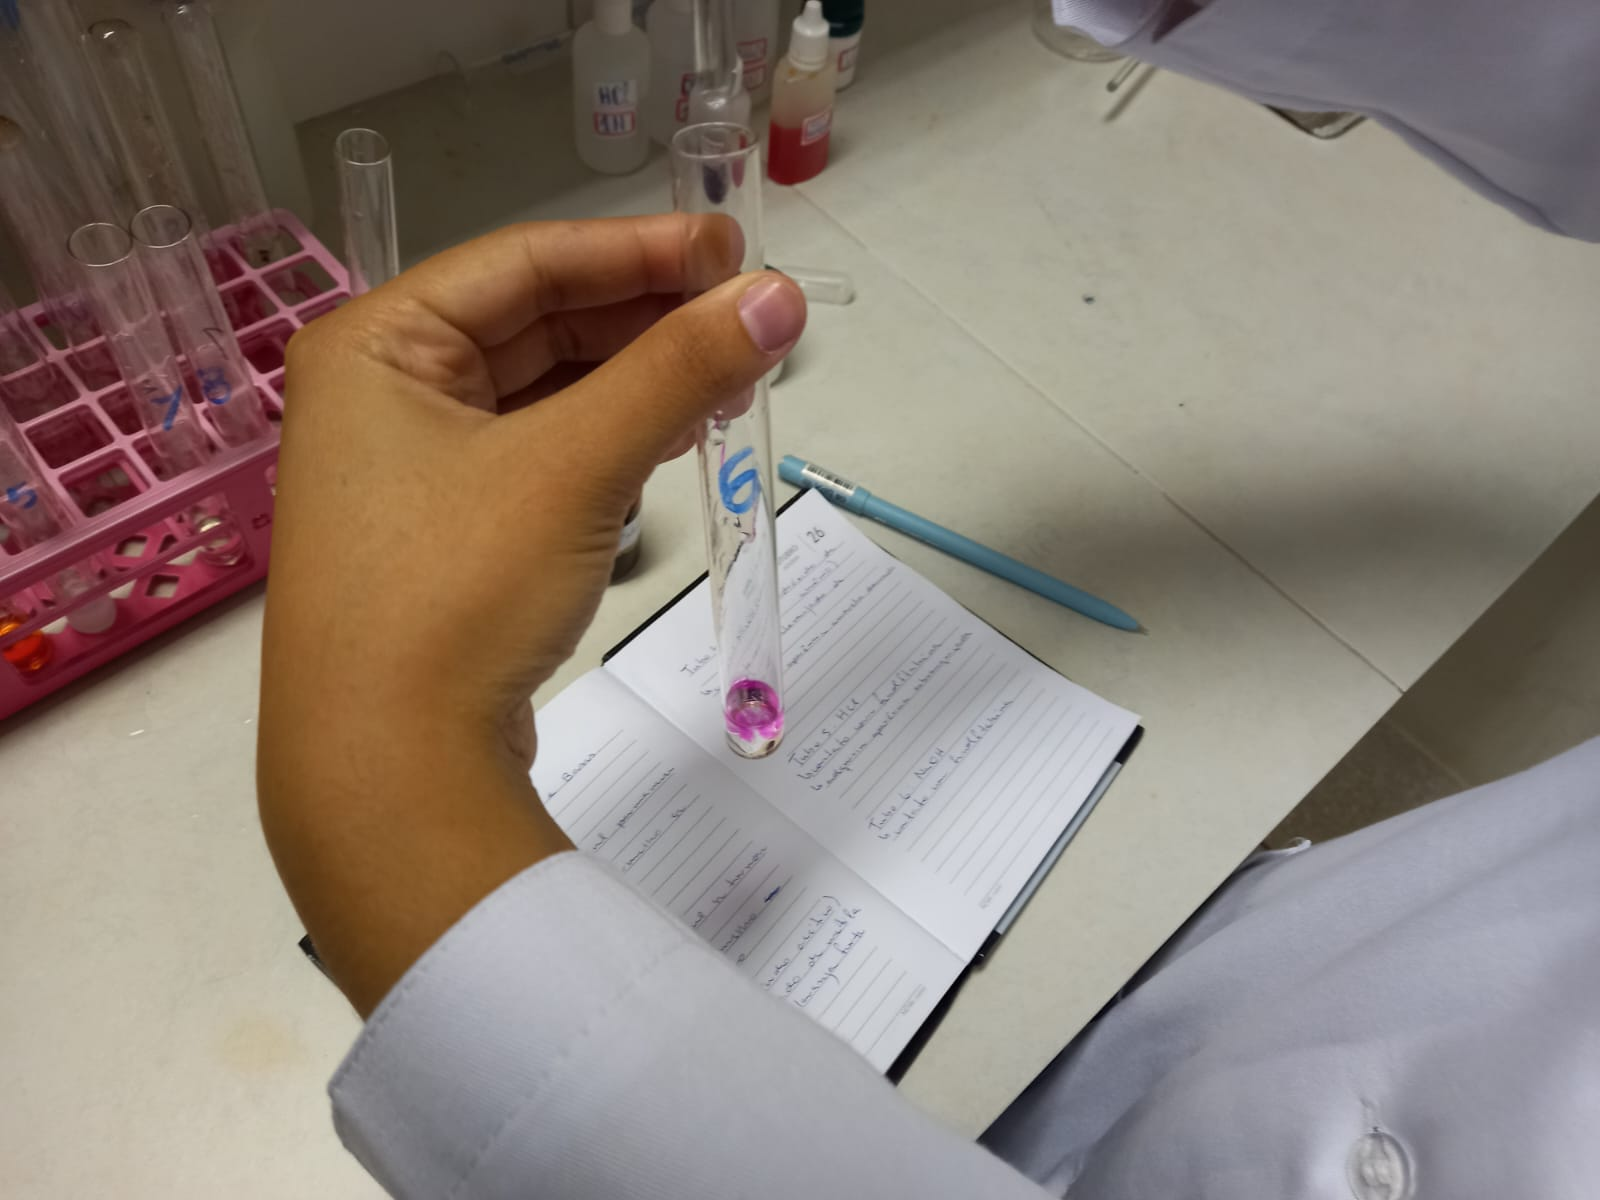
\includegraphics[scale=0.14]{pictures/tubo6pre.jpeg}}
            \qquad
            \subfloat[\centering A coloração apresentada pelo indicador foi incolor.\label{fig:figure12}]{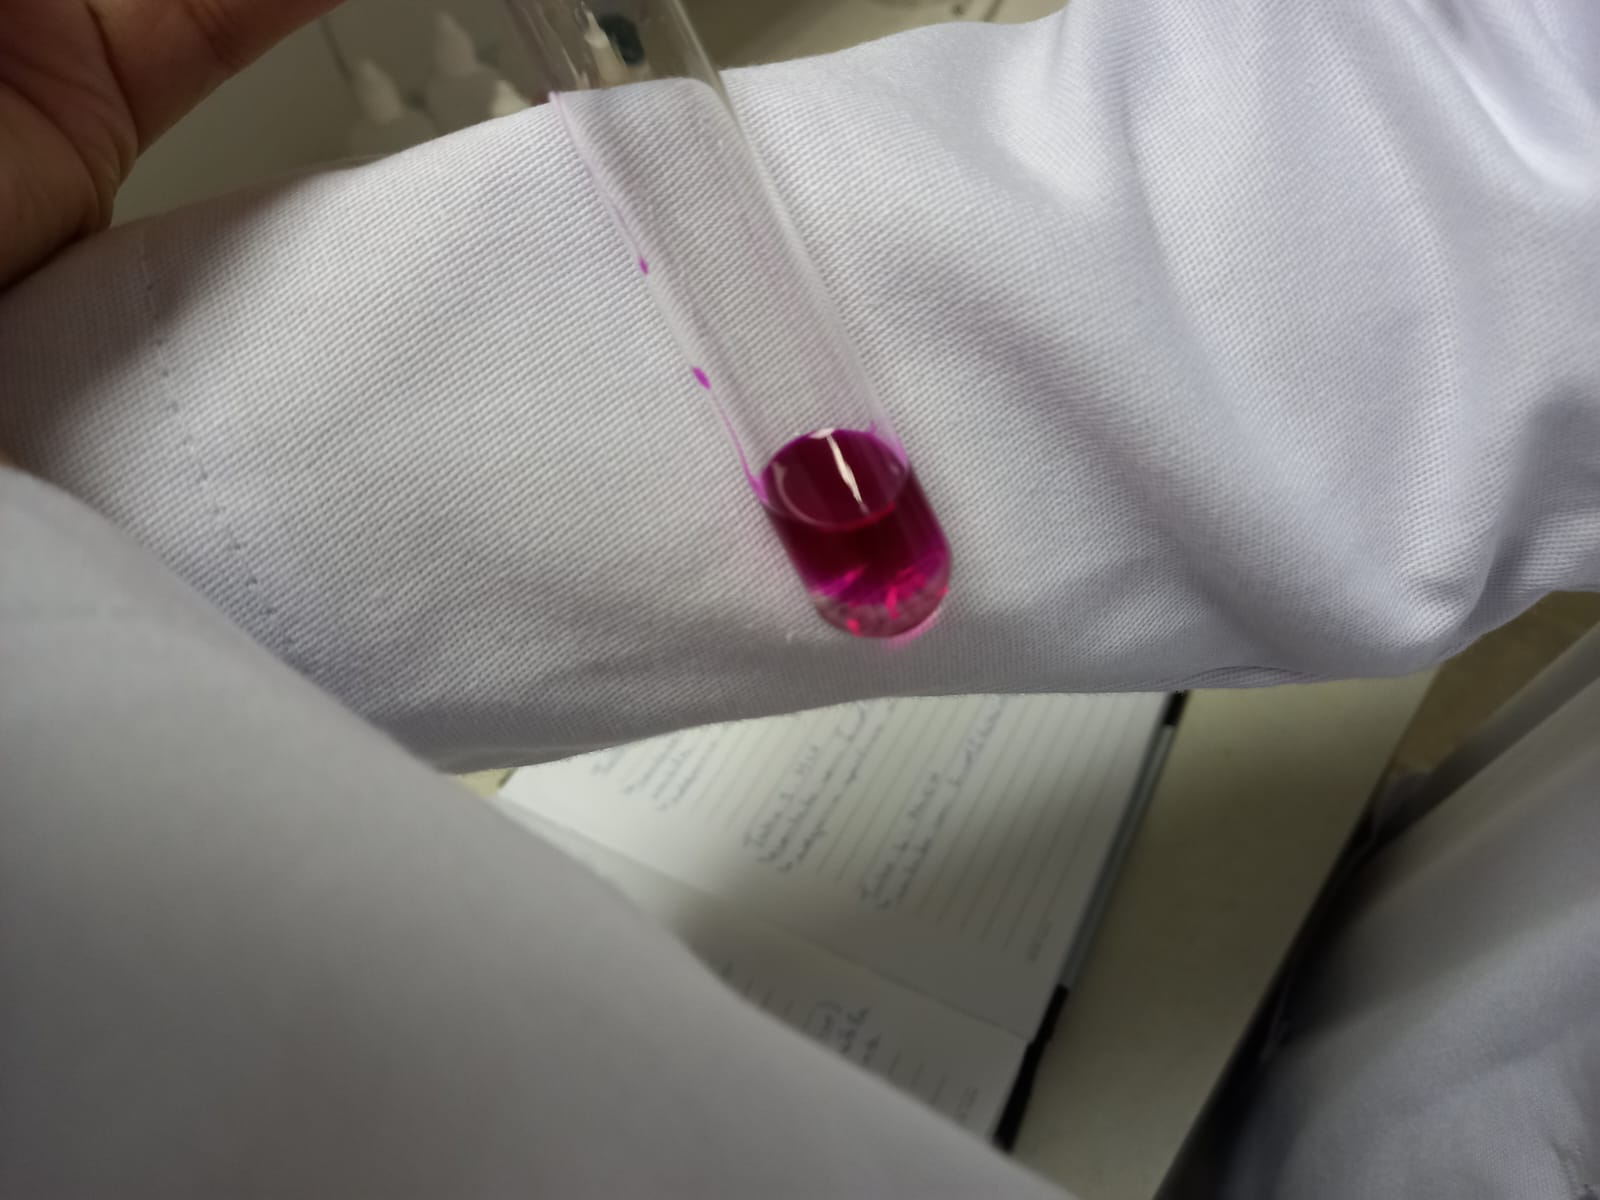
\includegraphics[scale=0.14]{pictures/tubo6pos.jpeg}}\label{fig:experimento15}
        \end{figure}

        \newpage

        \indent O sétimo tubo foi preparado com a solução de CH$_3$COOH 0,1 mol/L, e foi testado com o indicador de pH, o azul de bromotimol, o qual apresentou uma cor azul.

        \begin{figure}
            \centering
            \subfloat[\centering Teste do indicador de pH com a solução de CH$_3$COOH de 0,1 mol/L\label{fig:figure13}]{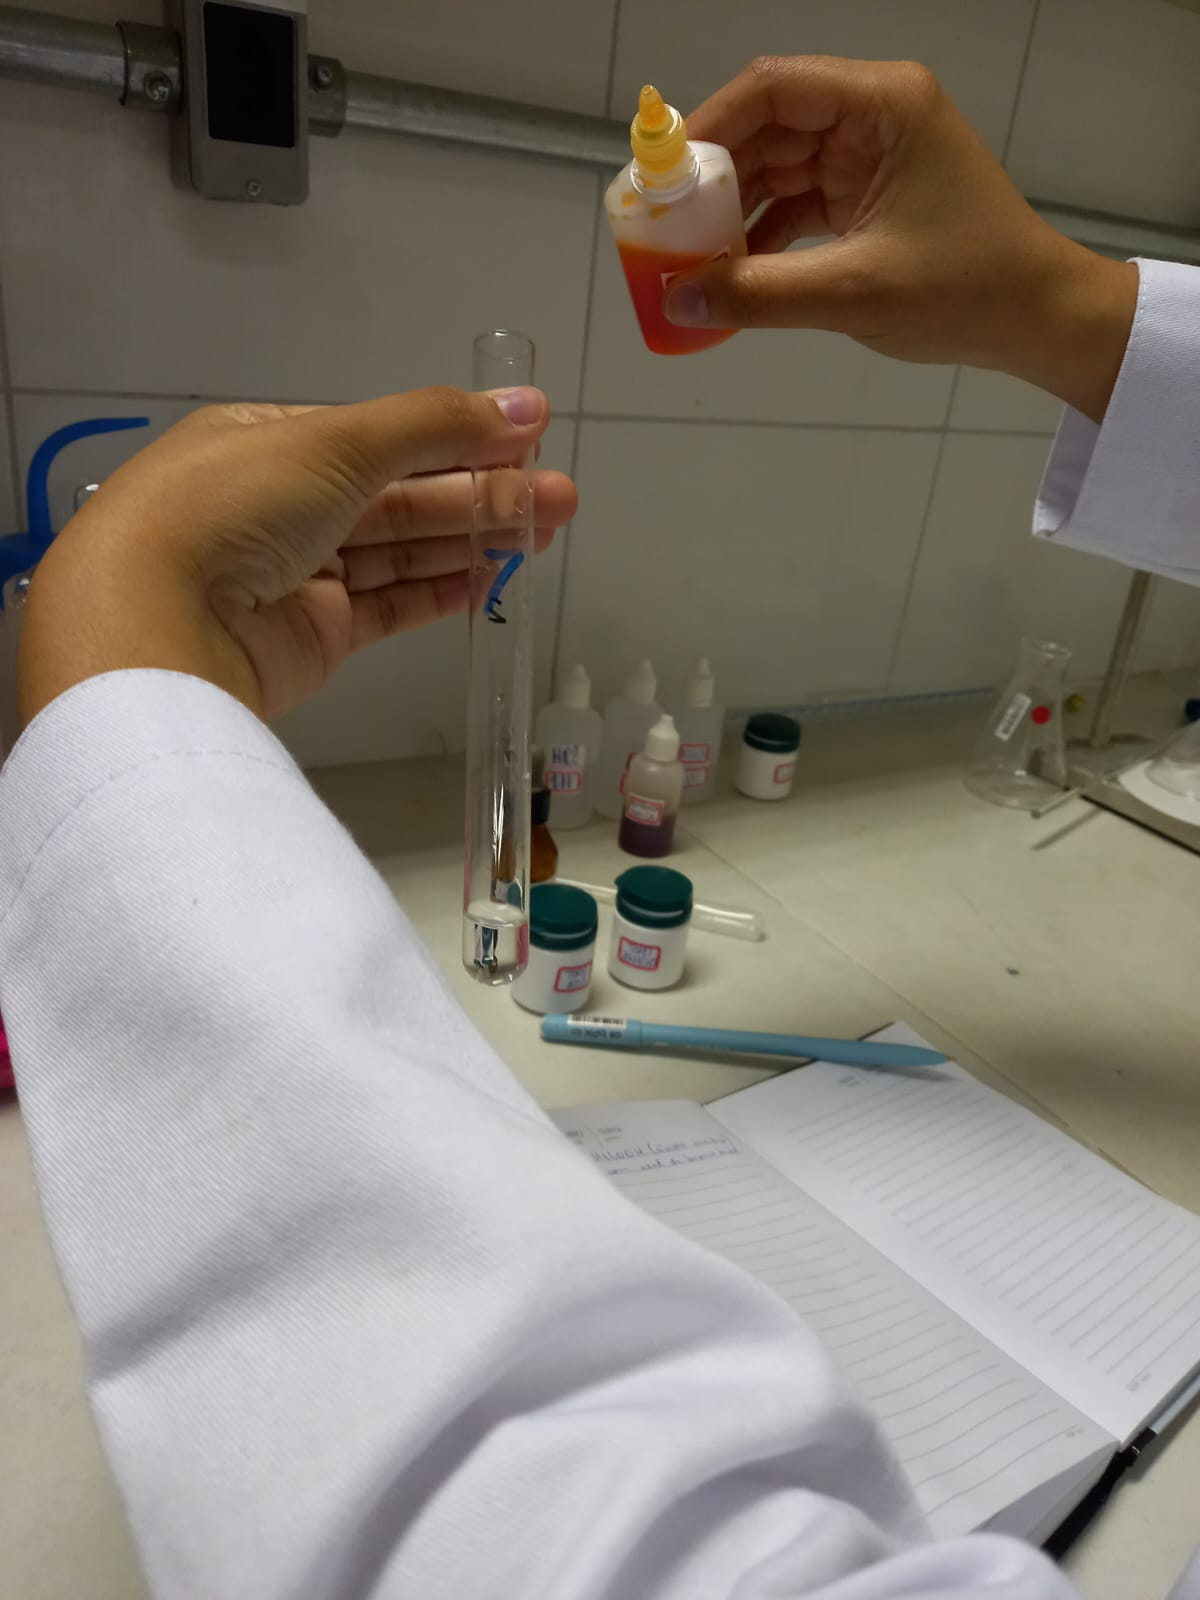
\includegraphics[scale=0.14]{pictures/tubo7pre.jpeg}}
            \qquad
            \subfloat[\centering A coloração apresentada pelo indicador foi azul.\label{fig:figure14}]{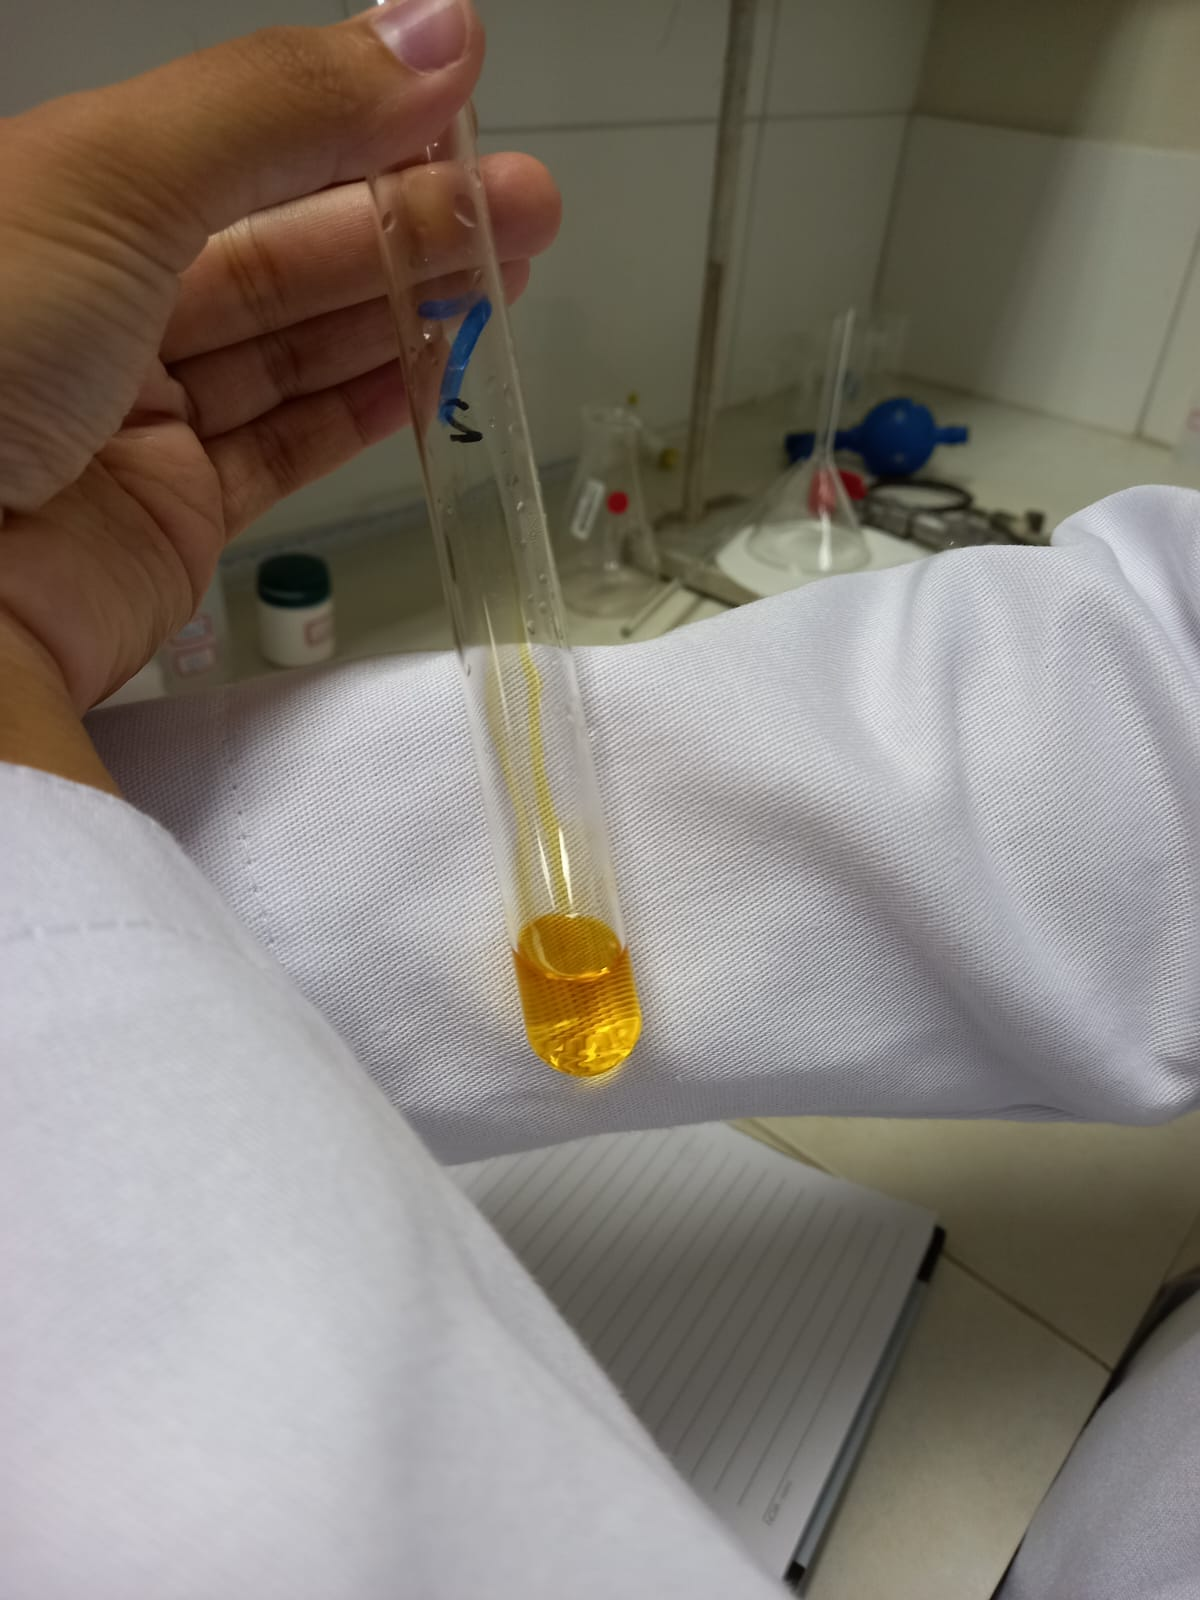
\includegraphics[scale=0.14]{pictures/tubo7pos.jpeg}}\label{fig:experimento16}
        \end{figure}

        \newpage

        \indent O oitavo tubo foi preparado com a solução de NH$_4$OH 0,1 mol/L, e foi testado com o indicador de pH, o azul de bromotimol, o qual apresentou uma cor amarela.

        \begin{figure}
            \centering
            \subfloat[\centering Teste do indicador de pH com a solução de NH$_4$OH de 0,1 mol/L\label{fig:figure15}]{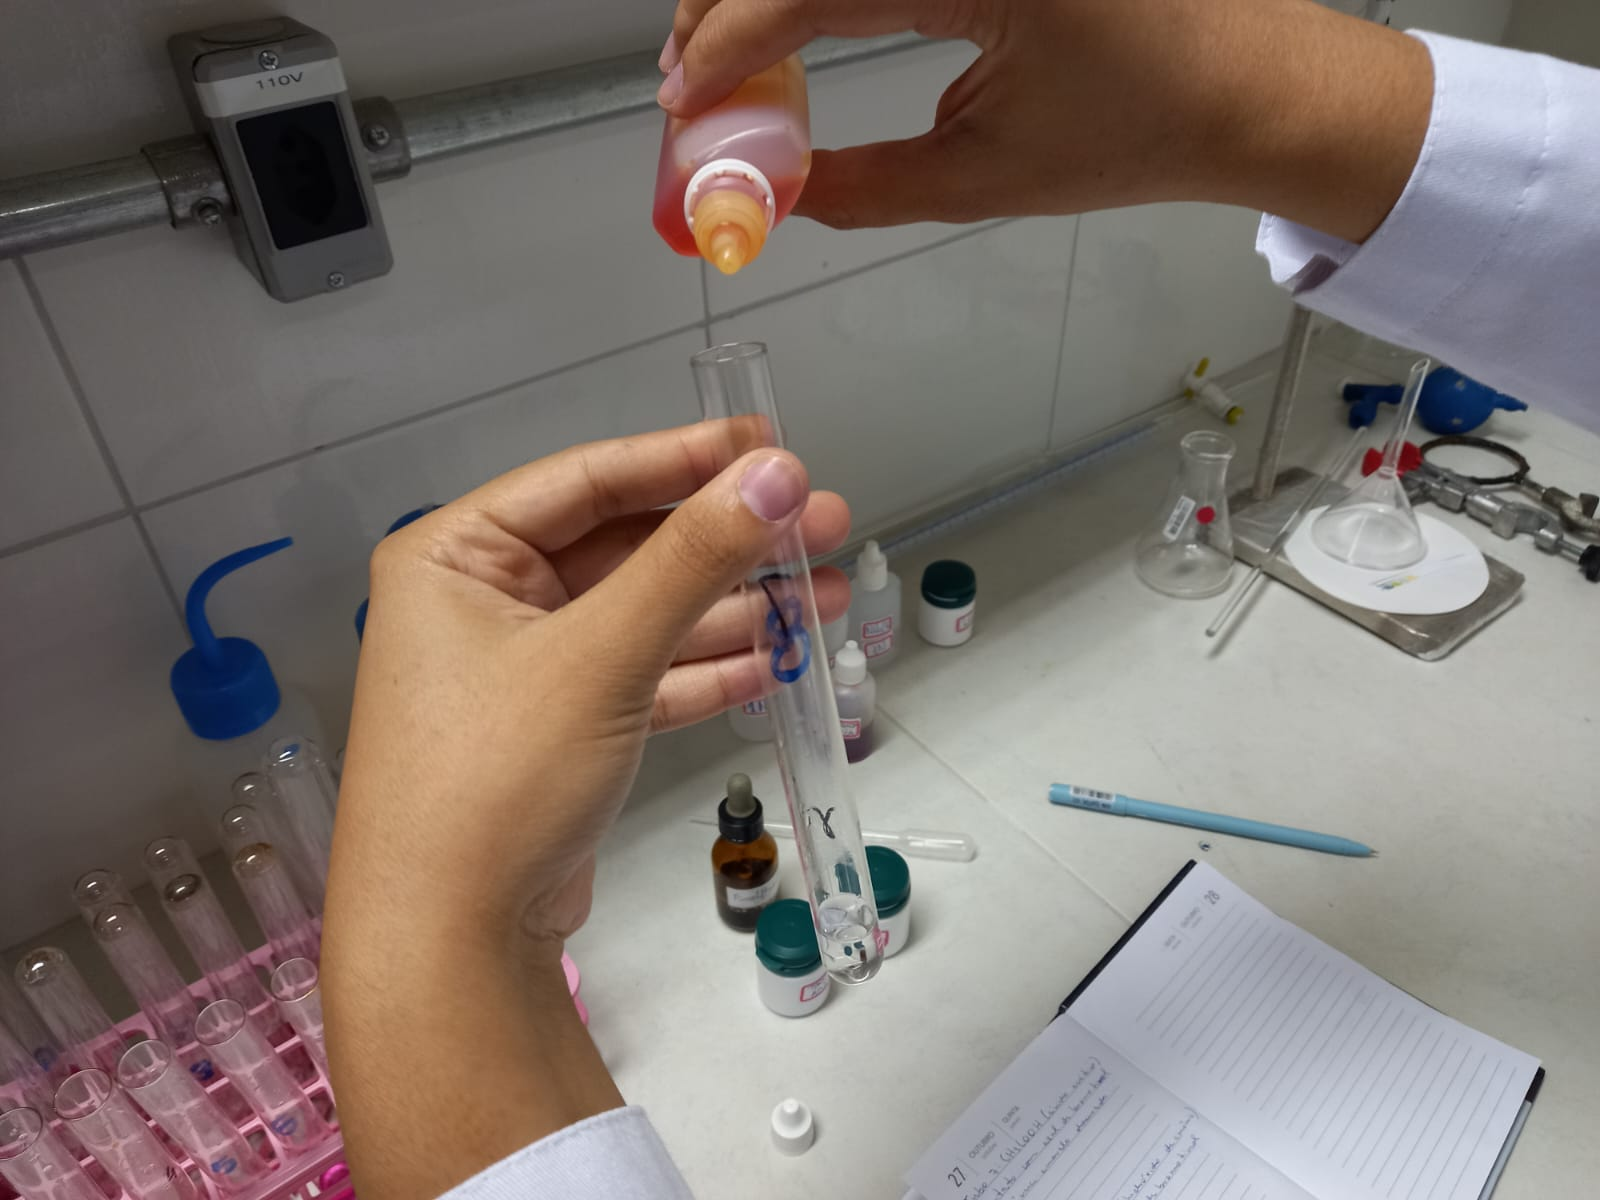
\includegraphics[scale=0.14]{pictures/tubo8pre.jpeg}}
            \qquad
            \subfloat[\centering A coloração apresentada pelo indicador foi amarela.\label{fig:figure16}]{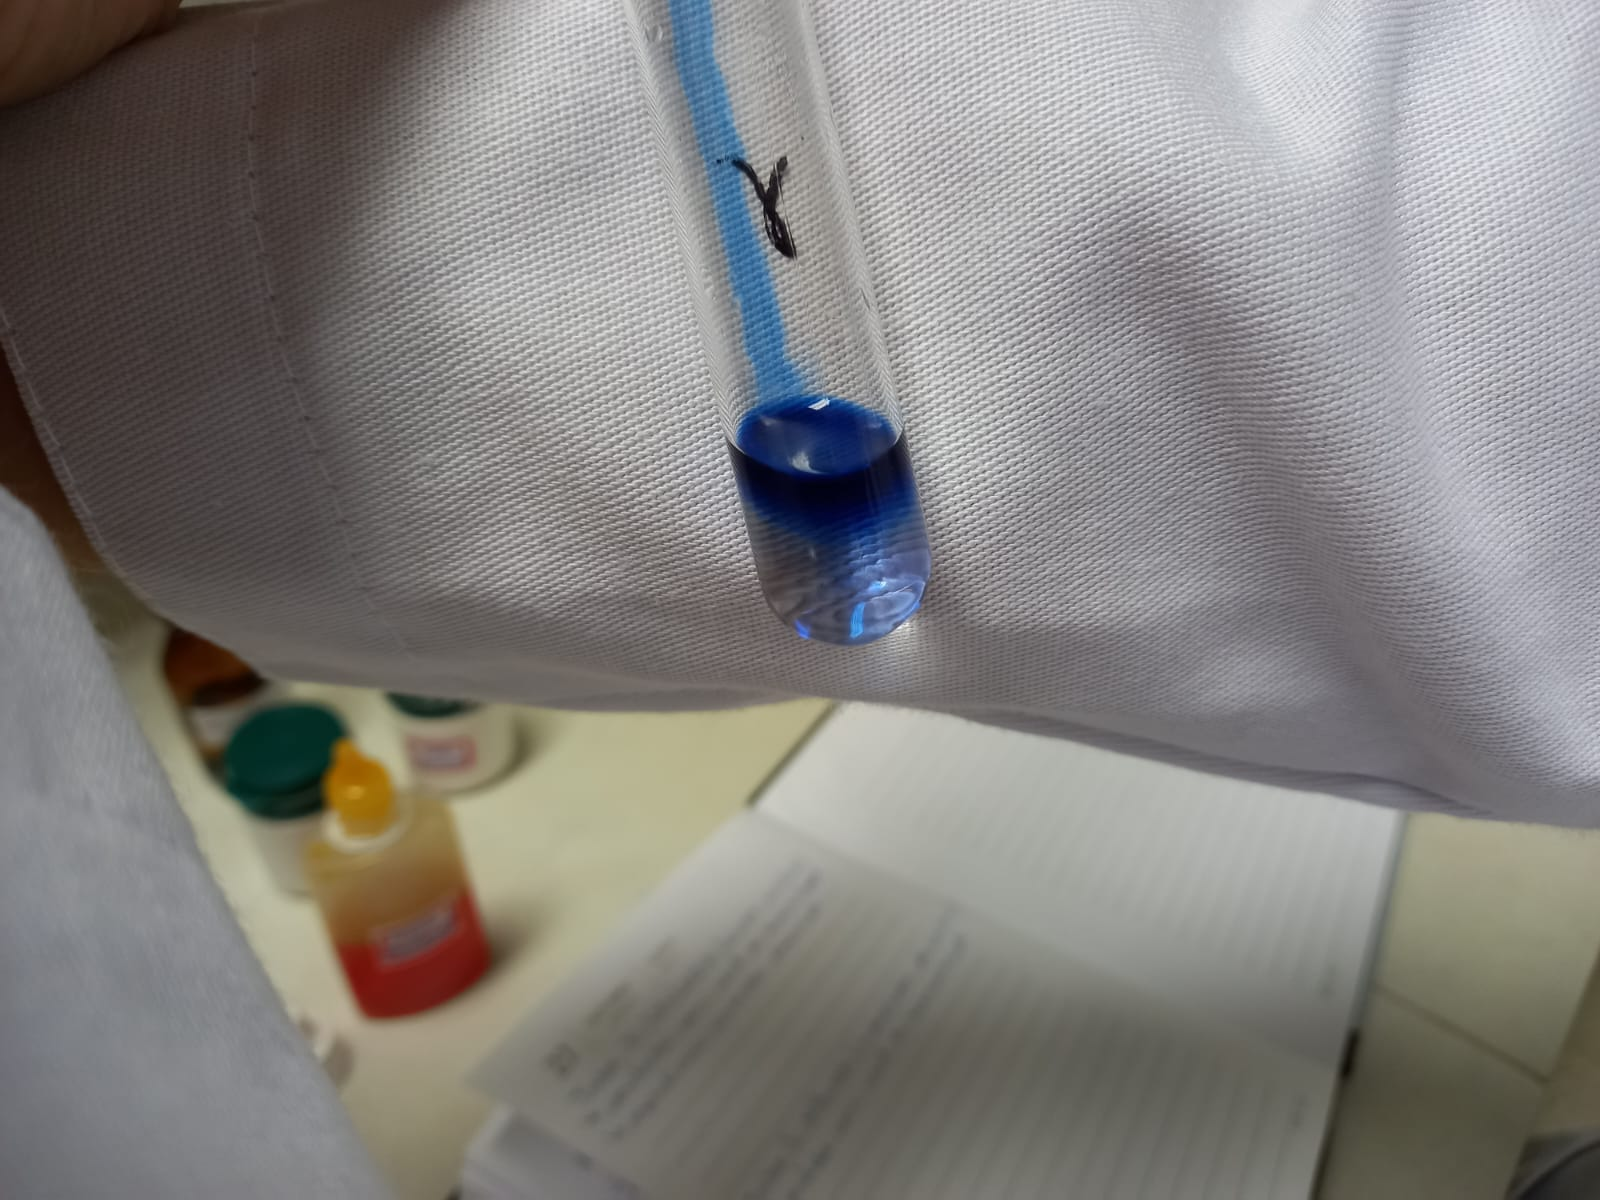
\includegraphics[scale=0.14]{pictures/tubo8pos.jpeg}}\label{fig:experimento17}
        \end{figure}

        \newpage

